\begin{enumerate}[font=\bfseries]

    \item \textbf{An image has 200x200 pixels. The image shows a 10x10 white
    square in the middle of the image and the background is black. Gaussian
    noise with a mean of 0.5 and variance of 0.01 is added to the image.}

    \begin{enumerate}[font=\bfseries, label=\alph*.]
	
	\item \textbf{In gaussian noise, what percentage of noise is within two
	standard deviations and one standard deviation?}

	Assuming that we are only talking about the gaussian noise distribution
	and not the image, these values are very well known. The probability
	that a random number is within two standard deviations of the mean is
	95\% and 68\% for one standard deviation.

	\item \textbf{What is the histogram before and after adding the noise?}

	I have written a matlab script to do this - please see the appendix. The
	histogram is:

	\begin{figure}[H]
	    \centering
	    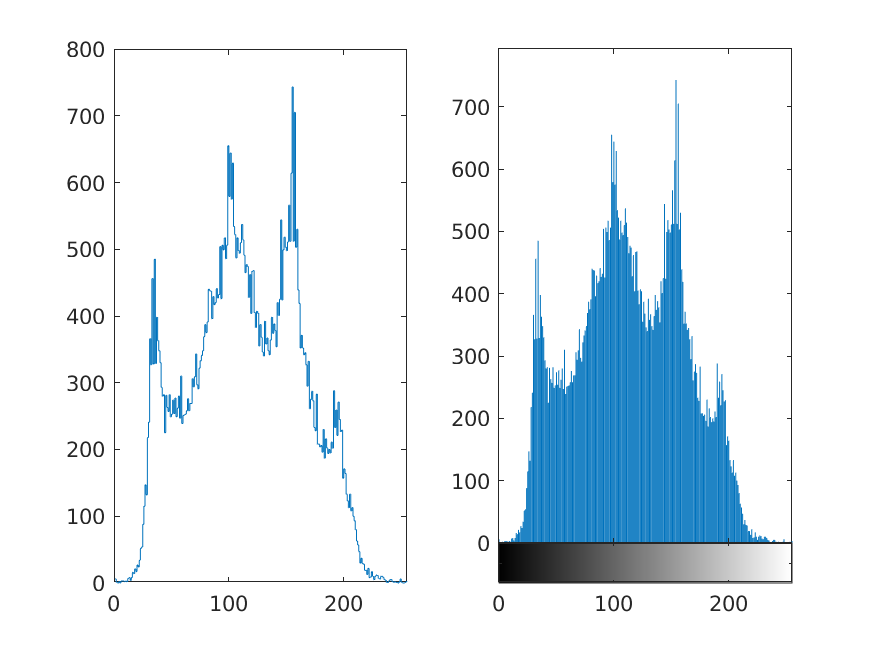
\includegraphics{addnoise.png}
	    \caption{Adding noise to an image}
	\end{figure}

	As you can see, we originally had all of our intensities at the minimum
	and maximum intensity values. It may look like there are no bins showing
	in the before image, but they are right at the edges since we have all
	the intensities at black and white. When we added noise, most of our
	pixels have a value of 0, so most of the noise is centered at 0.5 with
	the assigned variance. As for the small number of white pixels, I assume
	that the imnoise function wraps values above one to be within the range
	of 0 to 1. It is very possible that it doesn't, however if we were
	dealing with integer values and some sort of noise was added, the values
	would simply overflow. In this case, our noise would wrap around and
	still have an average value of 0.5.
    
    \end{enumerate}

    \item \textbf{An image, $f(x,y)$, and its FFT ,$F(u,v)$, are shown below,
    the noise functions a-d are added to the image and the Fourier transform of
    the degraded images are shown. Explain which one belongs to which.}

    The noise equations are labeled alphabetically and so I will label the
    fourier representations numerically starting from 0 from left to right. 

    Fourier representation 0 has the noise function d. The 2x and -2y terms add
    the high frequency harmonics seen in the top right and bottom left corners,
    and the x/4 and y/4 terms create the low frequency harmonics found in the
    top left and bottom right quadrants.

    Fourier representation 1 has the noise degradation function b. This simple
    noise creates harmonics in the top left and bottom right quatrants.

    Fourier representation 2 has the noise degradation function c. The only
    difference between c and b is that c has the -y term. This is essentially a
    negative frequency and culminates in a harmonic "flip" over the v axis.

    Fourier representation 3 has the noise degradation function a. Here we have
    harmonics due to the equally sized frequencies in the x and y direction, and
    then two more at the same frequency in the x axis, but higher frequency in
    the y axis.

    \item \textbf{Explain how contra harmonic operates if the area has constant
    values of P?}

    Assuming that "the area" is referencing the spatial filtering window, there
    will be no change in the resulting pixel. First, if the contra harmonic is
    set to behave as a mean filter, the average of a bunch of numbers that are P
    results in the value P. As for the harmonic filer, the same applies. If you
    calculate the result, the final value is P.

    \item \textbf{What is the difference between salt noise and pepper noise?
    Why are contra harmonic filters effective at eliminating salt noise when Q
    is positive and pepper noise when Q is negative?}

    Salt and pepper noise is a type of impulse noise seen in images. The
    histogram for this type of noise is made up of single high probability bins.
    This results in pixels in the original image making sharp changes to a high
    value (salt) or a low value (pepper) every once in a while depending on the
    noise type.

\end{enumerate}
